\documentclass{article}
\usepackage[utf8]{inputenc}
\usepackage[spanish,mexico]{babel}
\usepackage{amsthm}
\usepackage{amsmath}
\usepackage{amssymb}
\usepackage{amsfonts}
\usepackage{latexsym}
\usepackage{color}
\usepackage{graphics,graphicx,graphpap}
\usepackage{fullpage}
\usepackage{float}
\usepackage{tikz} 
\usepackage{hyperref}


\title{Machine Learning para detectar el riesgo de Cardiopatía Coronaria}
\author{José Ángel Godoy Santiago}
\date{Noviembre 2025}

\begin{document}

\begin{figure}[h]
		\raggedright
		
\includegraphics[scale=0.07]{Logo_UNAM.png} \hfill 
\includegraphics[scale=0.18]{Logo_P4.jpg}
    \end{figure}

    
\begin{center}
    {\Large \textbf{Machine Learning para detectar el riesgo de Cardiopatía Coronaria.}}\\
    \vspace{7.5mm}
	{\large Godoy Santiago José Ángel}\\
	\vspace{7.5mm}
    {\large Noviembre 2025}
\end{center}

\begin{center}
		\textcolor{teal}{\rule{150mm}{0.5mm}}
\end{center}	
    
\begin{abstract}
		\indent Este proyecto documenta el uso de algoritmos de Machine Learning (regresión logística y árboles de decisión) para predecir el riesgo de desarrollar cardiopatía coronaria en un periodo de 10 años. Utilizando un conjunto de datos clínicos del estudio de Framingham, se entrenaron los modelos para clasificar la presencia o ausencia de la enfermedad a partir de factores de riesgo como la edad, el nivel de colesterol y la presión sistólica.

        Al evaluar el rendimiento, ambos modelos alcanzaron una exactitud (accuracy) global aparentemente buena, rondando el 85\%. Sin embargo, un análisis estricto de las métricas demostró que este número es engañoso debido al fuerte desbalance en los datos originales. En realidad, los modelos presentaron un recall deficiente para la clase minoritaria; es decir, fallaron considerablemente al identificar a los pacientes que sí desarrollarán la enfermedad, ya que la tendencia matemática fue clasificar a la gran mayoría como "sanos".
        
        Se concluyó que, en contextos de diagnóstico médico, evaluar un modelo únicamente por su exactitud es un error estadístico. Se hace evidente la necesidad de implementar técnicas de balanceo de datos (como sobremuestreo) o ajustes en los umbrales de decisión para que el algoritmo tenga verdadera utilidad clínica y no arroje falsos negativos, lo cual queda establecido como la principal línea de trabajo a futuro.
	\end{abstract}

    \begin{center}
		\textcolor{teal}{\rule{150mm}{0.5mm}}
    \end{center}	

\section{Introducción}

El objetivo de este proyecto es predecir la presencia de cardiopatía coronaria o cardiopatía congénita mediante el uso de dos algoritmos de Machine Learning: regresión logística y árbol de decisión.
El conjunto de datos utilizado pertenece al dominio público, de acuerdo con \href{https://biolincc.nhlbi.nih.gov/teaching/}{\textit{National Heart, Lung, and Blood Institute}}, y se describe con mayor detalle en la Sección \ref{data}.

Este trabajo fue elaborado por estudiantes de los Estudios Técnicos Especializados en Computación de la Escuela Nacional Preparatoria Núm. 4 “Vidal Castañeda y Nájera”, en colaboración con la técnica académica \href{https://github.com/ingridmidory}{Ingrid Midory Monterroso Alfaro}, responsable del programa de Prácticas Profesionales “Data Minds. Laboratorio de Inteligencia Artificial” del mismo plantel.

%Datos: 
%https://biolincc.nhlbi.nih.gov/media/teachingstudies/FHS_Teaching_Longitudinal_Data_Documentation_2021a.pdf?link_time=2025-01-15_15:26:50.135928

    \subsection{Motivación}

    Las enfermedades cardíacas son un serio problema de salud pública, tan grande es su impacto que son la principal causa de muerte a nivel mundial¹, por ello, se necesitan de nuevas y mejoras formas de hacer frente a esta problemática que afecta a millones de personas alrededor del mundo, y los avances en la tecnología, específicamente en el área de la inteligencia artificial, pueden brindarnos herramientas valiosas que nos ayuden a detectar de forma temprana esta enfermedad en pacientes.

    \subsection{Objetivos}

    Predecir la ausencia o presencia de cardiopatía coronaria (CC o Coronary Heart Disease, CHD) en un periodo de 10 años mediante la aplicación de técnicas de aprendizaje automático (Machine Learning). Para ello se emplearán algoritmos de clasificación, específicamente regresión logística y árbol de decisión, los cuales permiten modelar la probabilidad de ocurrencia de un evento binario. En este caso, ambos modelos clasificarán los resultados en dos categorías —presencia o ausencia de la enfermedad—, lo que los convierte en herramientas adecuadas para comparar su eficiencia y desempeño en la predicción de la cardiopatía coronaria. La base de datos utilizada se encuentra disponible para uso público a través del National Heart, Lung, and Blood Institute.      

%\newpage

\section{Preliminares}

La inteligencia artificial (IA) son aquellos programas informáticos que intentan imitar la inteligencia humana, de esta forma, puede facilitarse y agilizarse la realización de diversas tareas que en condiciones ordinarias requerirían de la intervención de un ser humano. Dentro de esta área, se encuentra el Machine Learning, o aprendizaje automático, una rama de la IA que busca que los sistemas sean capaces de realizar una tarea y mejorar su desempeño a partir de una determinada cantidad de datos proporcionados, sin necesidad de ser programados de manera explícita para cada caso.

En este contexto, el Machine Learning adquiere un papel fundamental, ya que permite construir modelos capaces de identificar patrones complejos dentro de grandes volúmenes de información. Gracias a este enfoque, los sistemas no solo ejecutan instrucciones predefinidas, sino que aprenden de los datos y ajustan su comportamiento conforme reciben nueva información. A continuación, se describe con mayor detalle el funcionamiento y las características principales del Machine Learning.

Para comprender mejor el funcionamiento del Machine Learning y su aplicación en el análisis de datos médicos, es necesario distinguir entre los principales enfoques de aprendizaje utilizados. Cada uno de ellos se basa en una forma distinta de organizar y aprovechar la información disponible, lo que determina el tipo de problemas que pueden abordarse y los resultados que se obtienen. En particular, a continuación se describen los métodos de aprendizaje supervisado y aprendizaje no supervisado, así como sus características y aplicaciones más relevantes.

    \subsection {Machine Learning}
    
    El Machine Learning o aprendizaje automático es una disciplina de la inteligencia artificial que permite a las máquinas aprender y mejorar su desempeño a partir del análisis de grandes volúmenes de datos, mediante la identificación de patrones relevantes. En lugar de seguir instrucciones programadas de manera explícita, estos sistemas ajustan su comportamiento con base en la información que se les proporciona. Dentro de esta área existen diversos algoritmos, entre los cuales destacan principalmente los de aprendizaje supervisado y aprendizaje no supervisado, que se diferencian por la forma en que utilizan los datos durante el proceso de entrenamiento.

    \subsection{Aprendizaje Supervisado}
    
    En los algoritmos de aprendizaje supervisado, el modelo es entrenado utilizando conjuntos de datos que incluyen tanto las variables de entrada (\textit{input}) como las variables de salida (\textit{output}). Es decir, los datos se encuentran previamente etiquetados, lo cual permite al modelo aprender la relación entre entradas y salidas; de ahí que este enfoque reciba el nombre de aprendizaje supervisado.

    Dentro del aprendizaje supervisado existen diversos algoritmos ampliamente utilizados, los cuales pueden clasificarse, de manera general, en métodos de regresión y clasificación. Entre los más comunes se encuentran la regresión lineal, empleada para predecir valores continuos; la regresión logística, utilizada en problemas de clasificación binaria; entre otros algoritmos. La elección del algoritmo depende del tipo de problema, de la naturaleza de los datos y del objetivo del análisis.
        
        \subsubsection{Regresión lineal y regresión logística}
        
        La regresión lineal es un método estadístico el cual predice valores que podrían encontrarse sobre una línea recta, la cual se ajusta sobre los datos de entrada y salida con los que se entrena el modelo. En otras palabras, esta técnica encuentra una relación lineal entre las variables dependientes e independientes.
        
        Se considera que la variable $X$ es la variable independiente que por lo general cambia a lo largo del tiempo, mientras que la variable $Y$ es la variable dependiente de cada valor de $x_i$ de $X$

        La siguiente gráfica nos muestra cada valor $y_i$ observado para un $x_i$ lo podemos ver como el valor esperado de $Y$ dado $x_i$ más un error. 

            \begin{figure}[H]
                \centering
                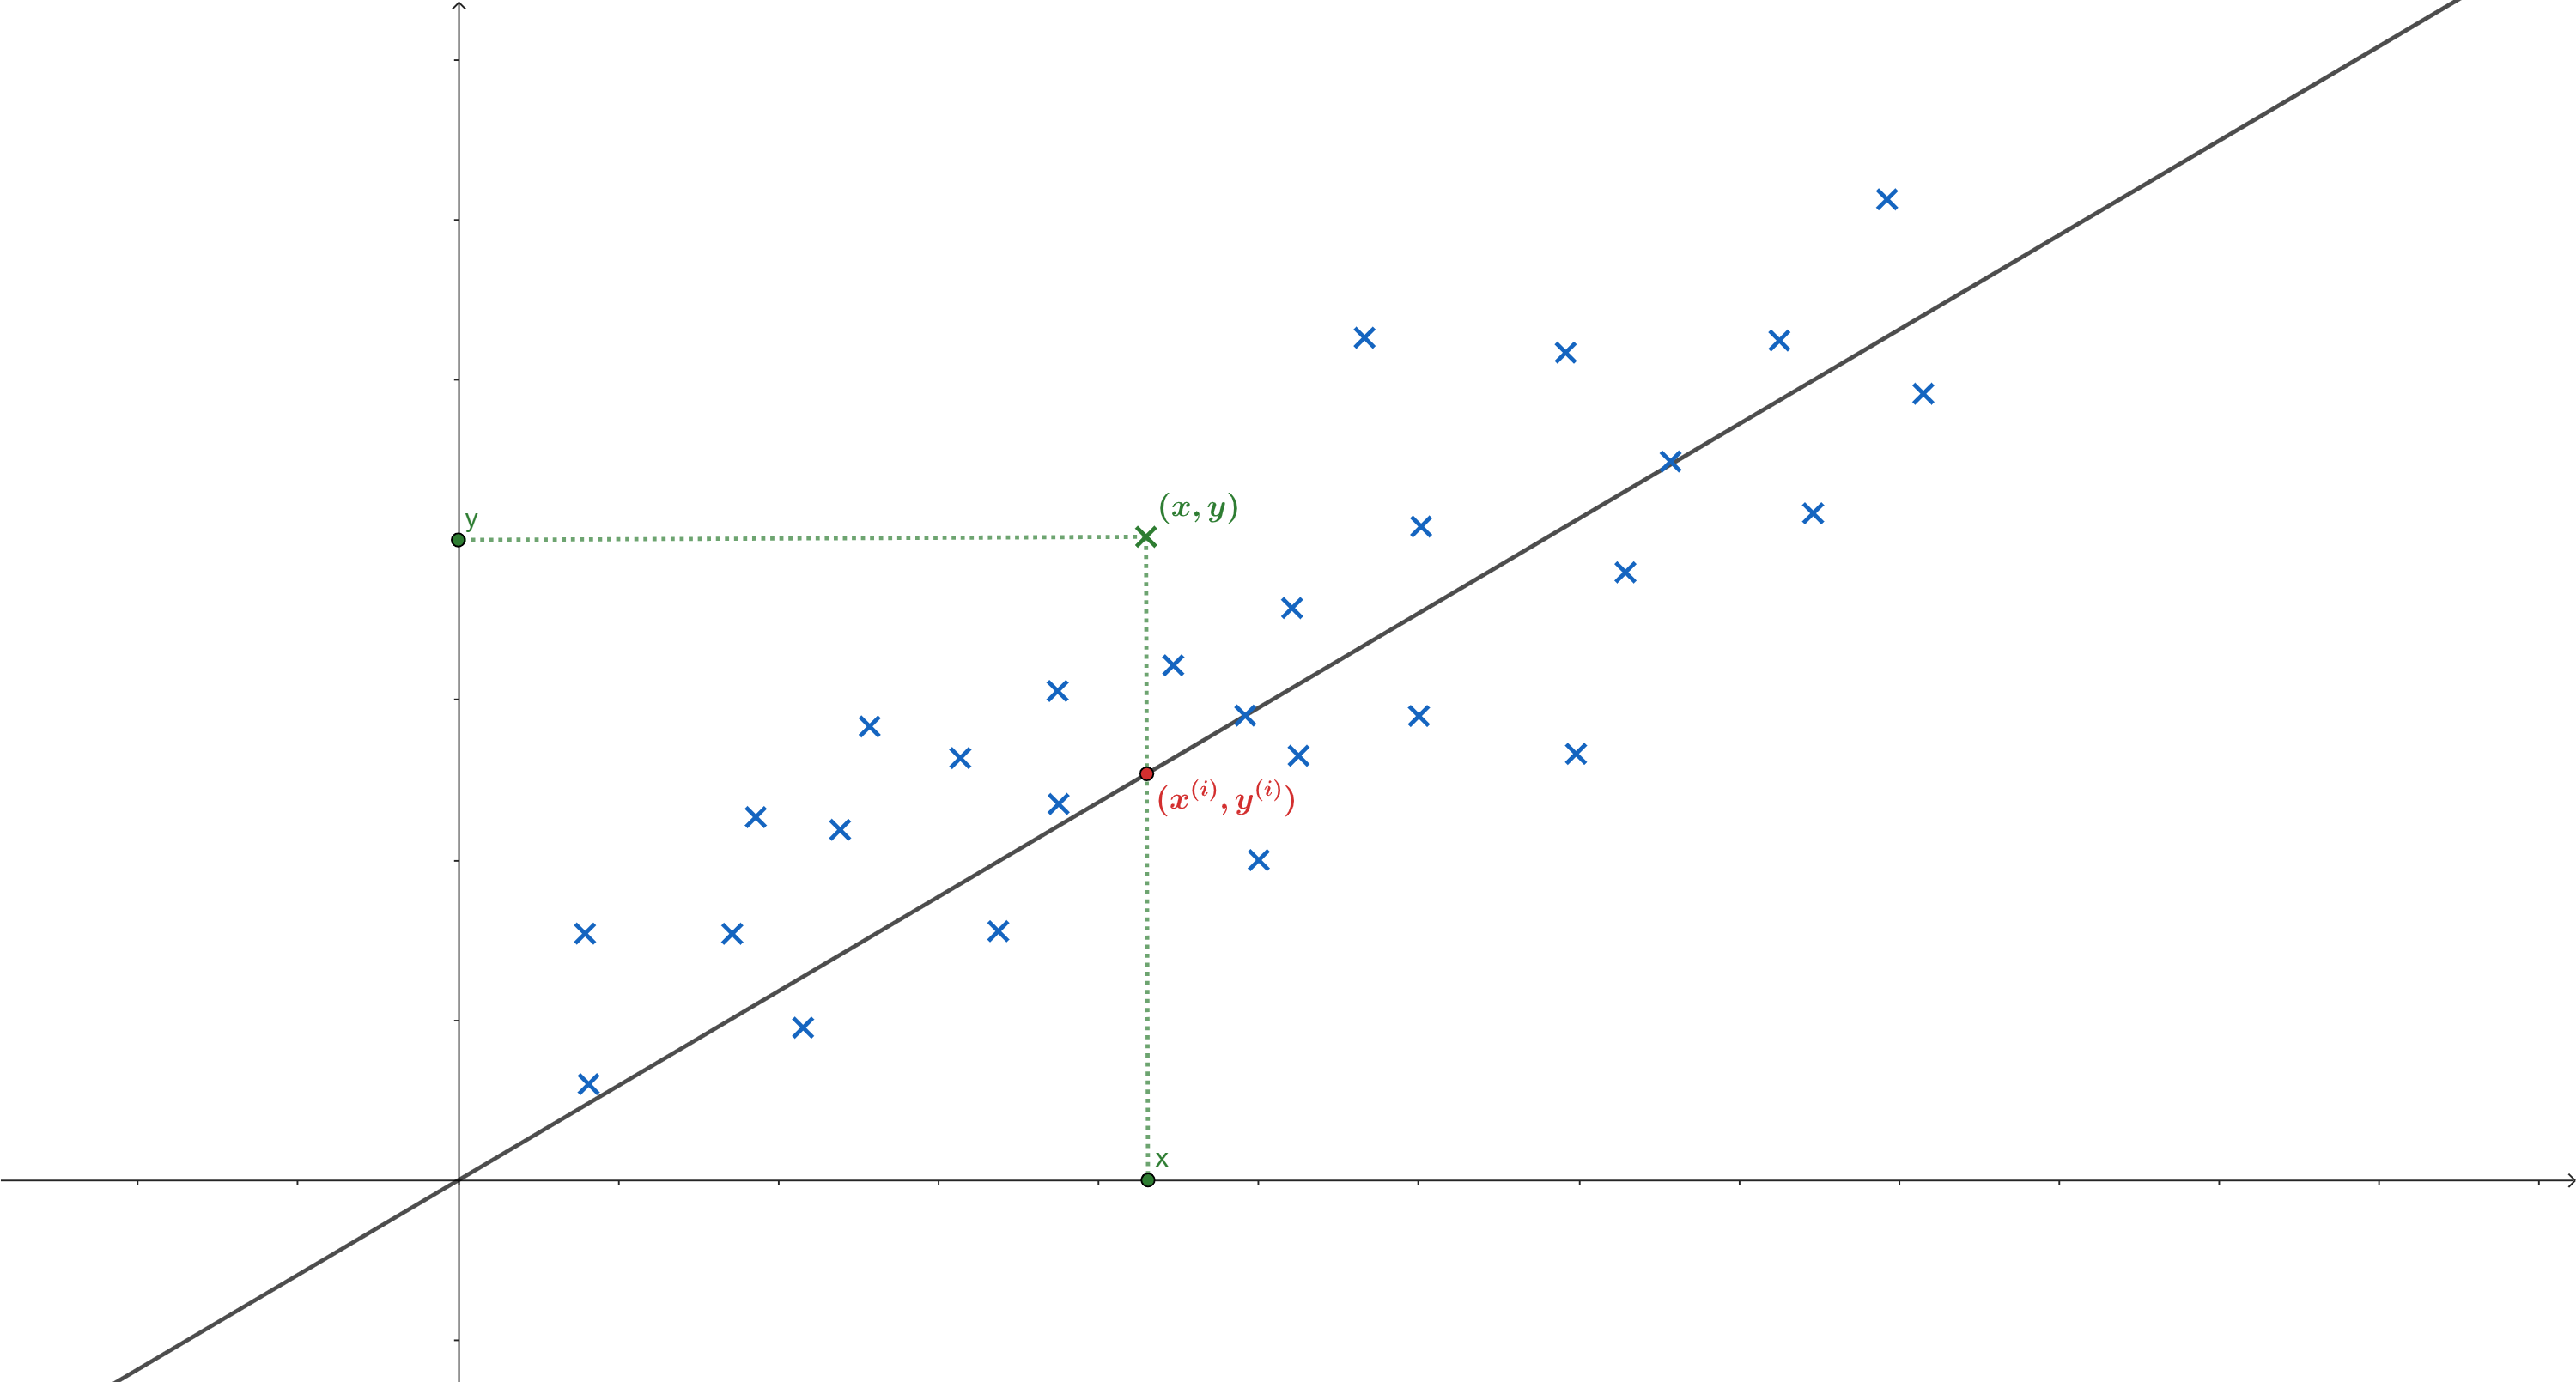
\includegraphics[width=0.80\linewidth]{Regresión lineal.png}
                \caption{Regresión lineal.}
                \label{fig:placeholder}
            \end{figure}
            
        El modelo de regresión lineal simple el que se representa de la siguiente manera:

        \begin{equation}
            f_{w,b}(x) = wx + b
        \end{equation}
        
        Donde:
        \begin{itemize}
            \item $w$ (peso o \textit{weight}): representa el parámetro que el modelo multiplica por la variable de entrada, indicando la fuerza de la relación.
            \item $x$: es la variable independiente o dato de entrada.
            \item $b$ (sesgo o \textit{bias}): es el término independiente que permite desplazar la línea de ajuste, representando el valor de la predicción cuando $x = 0$.
        \end{itemize}

        En la regresión logística, el modelo predice la categoría de una variable en base a la identificación de las relaciones entre los datos de entrada y salida brindados previamente. Este método hace uso de curvas para predecir estas categorías.
        En la regresión logística, el modelo predice la categoría de una variable con base en la identificación de las relaciones existentes entre los datos de entrada y la variable de salida previamente proporcionados. Este método hace uso de la función sigmoide, una curva con forma de “S” que transforma una combinación lineal de las variables de entrada en un valor comprendido entre 0 y 1, el cual puede interpretarse como una probabilidad. A partir de esta probabilidad, el modelo asigna una categoría final, lo que lo hace especialmente adecuado para problemas de clasificación binaria, como la detección de la presencia o ausencia de enfermedades cardiovasculares.

        Para la regresión logística, se utiliza la función sigmoide, la cual transforma la salida en un valor de probabilidad entre 0 y 1:

        \begin{equation}
            f_{w,b}(x) = \frac{1}{1 + e^{-z}}
        \end{equation}
        
        Donde:
        \begin{itemize}
            \item $z = wx + b$: es la combinación lineal de los datos de entrada con sus respectivos pesos y el sesgo.
            \item $e$: es la constante matemática (número de Euler).
        \end{itemize}

            \begin{figure}[H]
                \centering
                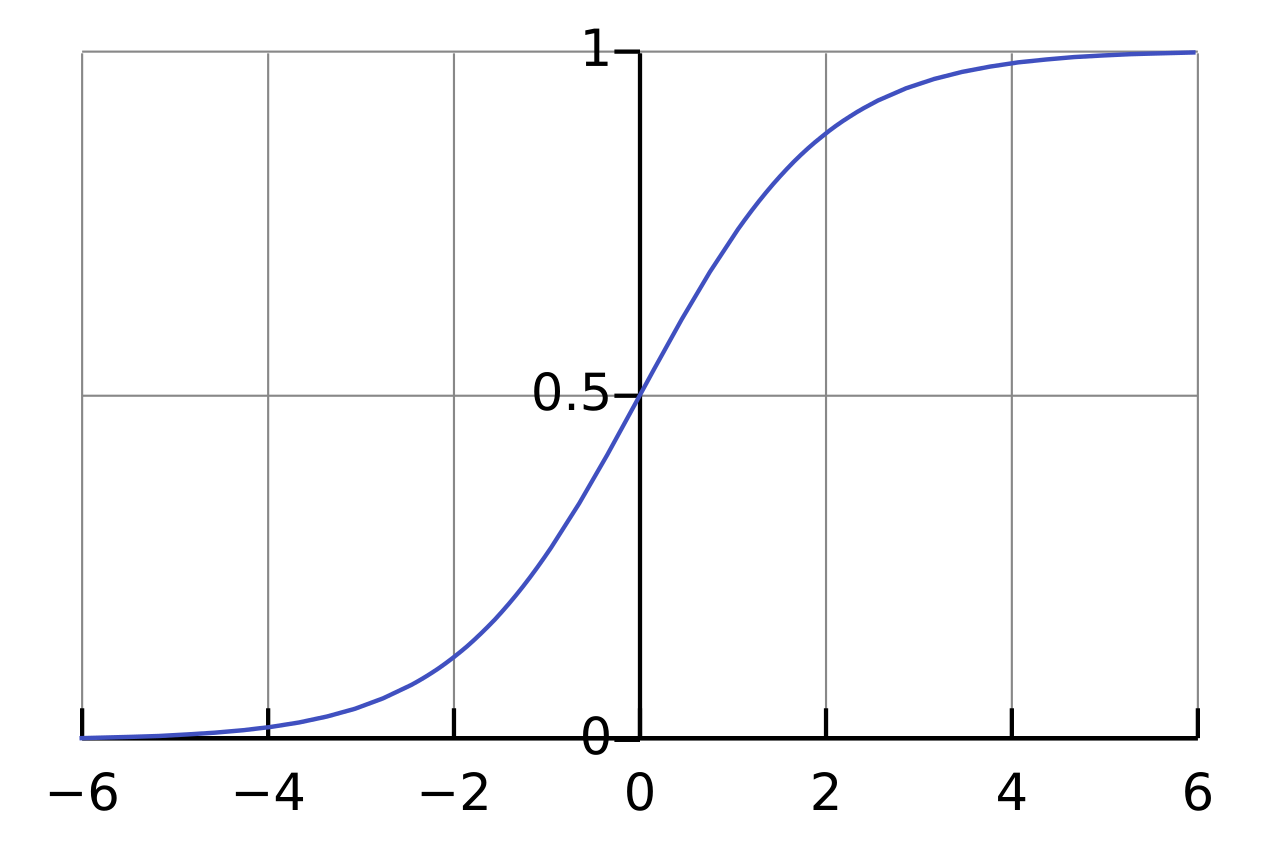
\includegraphics[width=0.50\linewidth]{Logistic-curve.svg.png}
                \caption{Función Sigmoid.}
                \label{fig:placeholder}
            \end{figure}

        \subsubsection{Árbol de decisión}

        Los árboles de decisión, como su nombre lo indica, utilizan una estructura jerárquica similar a la de un árbol para tomar decisiones basadas en los atributos o características de los datos de entrada. Estas estructuras de datos están compuestas por nodos, que representan las decisiones o preguntas que el algoritmo evalúa; ramas, que corresponden a las posibles respuestas o consecuencias de dichas decisiones; y nodos hoja, en los cuales se obtiene el resultado final o la predicción del modelo. Los árboles de decisión permiten modelar relaciones no lineales de manera intuitiva y son ampliamente utilizados debido a su facilidad de interpretación y a su aplicabilidad en problemas de clasificación y regresión.
           
        A diferencia de la regresión logística, que modela la probabilidad de pertenencia a una clase mediante una función sigmoide y una combinación lineal de las variables de entrada, los árboles de decisión realizan la clasificación a partir de una secuencia de reglas condicionales. Mientras que la regresión logística asume una relación aproximadamente lineal entre las variables y el logaritmo de las probabilidades, los árboles de decisión pueden capturar relaciones no lineales y complejas de forma más flexible. No obstante, la regresión logística suele ofrecer una mayor estabilidad y facilidad de interpretación estadística, especialmente cuando se trabaja con conjuntos de datos bien estructurados.
        En conjunto, los algoritmos de aprendizaje supervisado constituyen herramientas fundamentales dentro del Machine Learning para el análisis y la predicción a partir de datos etiquetados. Métodos como la regresión logística y los árboles de decisión permiten abordar problemas de clasificación desde enfoques distintos, cada uno con ventajas y limitaciones particulares. El conocimiento de estas técnicas proporciona la base teórica necesaria para el desarrollo e implementación de modelos orientados a la detección de enfermedades cardiovasculares, objetivo principal del presente trabajo.
  
    \subsection{Aprendizaje No Supervisado}

    En los algoritmos de aprendizaje no supervisado, únicamente se proporcionan los datos de entrada, sin contar con etiquetas asociadas a una variable de salida. En este caso, el modelo tiene la tarea de identificar de manera autónoma las relaciones, estructuras o patrones existentes dentro de los datos, tales como agrupamientos o similitudes entre las observaciones.
    Dentro del aprendizaje no supervisado existen diversos algoritmos orientados al descubrimiento de patrones y estructuras ocultas en los datos. Entre los más utilizados se encuentran los métodos de agrupamiento como k-means, el clustering jerárquico y DBSCAN, así como técnicas de reducción de dimensionalidad como el análisis de componentes principales (PCA). Estos algoritmos son ampliamente empleados para la segmentación de datos y el análisis exploratorio. Sin embargo, dado que el presente trabajo se centra en la detección de enfermedades cardiovasculares mediante técnicas de clasificación, dichos métodos no serán descritos con mayor detalle, ya que no se utilizan en el desarrollo de este proyecto.

\section{Detección del riesgo de enfermedad coronaria a diez años}

 Se usará Google Colab para ejecutar el modelo de regresión logística y árbol de decisión, usando el lenguaje de programación Python. Podrá encontrar el código en los siguientes enlaces: \href{https://colab.research.google.com/drive/189_8BEiUsl_2C4G_fp8kIsU-RrV1-en2?usp=sharing}{Heart Disease Prediction Using Logistic Regression} y \href{https://colab.research.google.com/drive/1tWzOxwN4WQCwvuAscs4Zvb3vFKrXvqqG?usp=sharing}{Heart Disease Prediction Using Decision Tree}. Los datos sobre el CC o CHD fueron obtenidos de un estudio realizado a los habitantes de la ciudad de Framingham, Massachusetts. Este estudio fue realizado con la finalidad de conocer la causalidad de las enfermedades cardiovasculares en la comunidad de Framingham. Dicho conjunto de datos que utilizaremos para realizar el análisis y construir un modelo de agrupación se encuentra disponible para uso público en \href{https://biolincc.nhlbi.nih.gov/teaching/}{\textit{National Heart, Lung, and Blood Institute}}.

    \subsection{Análisis exploratorio de los datos}\label{data}

    Se usará información de código abierto de los residentes de la ciudad de Framingham, Massachusetts. El conjunto de datos proporciona diversa información de los pacientes, incluye más de 4.000 registros y 15 atributos. Se cuenta con 15 variables de entrada, las cuales son \textbf{male}, \texttt{age}, \textbf{education}, \texttt{currentSmoking}, \texttt{cigsPerDay}, \texttt{BPMeds}, \texttt{prevalentStroke}, \texttt{prevalentHyp}, \texttt{diabetes}, \texttt{totChol}, \texttt{sysBP}, \texttt{diaBP}, \texttt{BMI}, \texttt{hertrate} y \texttt{glucose}; así como  una variable de salida \texttt{TenYearCHD}, la cual nos indica si el paciente tiene riesgo de presentar la enfermedad dentro de los próximos 10 años.

    \begin{table}[h]
        \centering
        \begin{tabular}{|c|c|c|c|}
            \hline
            \textbf{Variable} & \textbf{Descripción} & \textbf{Tipo de dato} & \textbf{Tipo de variable} \\ \hline
            male & Sexo (0= mujer, 1= hombre) & Binaria  & Cualitativa\\ \hline
            age & Edad & Entero & Cuantitativa \\ \hline
            education &  Nivel educativo (1-4) & Entero & Cualitativa \\ \hline
            currentSmoking & Fumador frecuente (0=no, 1=sí) & Binaria  & Cualitativa \\ \hline
            cigsPerDay & Cigarros por día  & Numérica & Cuantitativa \\ \hline
            BPMeds & Medicación para la presión (0=no, 1=sí) & Binaria & Cualitativa \\ \hline
            prevalentStroke & Derrames cerebrales (0=no, 1=sí) & Binaria & Cualitativa \\ \hline
            prevalentHyp & Hipertensión (0=no, 1=sí) & Binaria & Cualitativa \\ \hline
            diabetes & Diabetes (0=no, 1=sí)  & Binaria & Cualitativa \\ \hline
            totChol & Nivel de colesterol & Numérica & Cuantitativa \\ \hline
            sysBP & Presión sistólica  & Numérica & Cuantitativa \\ \hline
            diaBP & Presión diastólica  & Numérica & Cuantitativa \\ \hline
            BMI & Indice de masa corporal & Numérica & Cuantitativa \\ \hline
            heartRate & Frecuencia cardiaca & Numérica & Cuantitativa \\ \hline
            glucose & Glucosa & Numérica & Cuantitativa \\ 
            \hline
            TenYearCHD & Presencia de enfermedad (0=no, 1=sí) & Binaria & Cualitativa\\ \hline
        \end{tabular}
        \caption{Tabla de datos.}
        \label{tab:mi_tabla}
    \end{table}

    Las estadísticas descriptivas permiten obtener una visión general de las características de la muestra utilizada en el estudio. En total, se analizaron 4,240 registros con diversas variables clínicas y demográficas. La edad promedio de los participantes fue de aproximadamente 49.6 años, con un rango entre 32 y 70 años. El 42.9 \% correspondió a hombres y cerca del 49 \% eran fumadores activos, con un promedio de 9 cigarrillos por día. En cuanto a las condiciones médicas, un 31 \% presentaba hipertensión y un 2.6 \% diabetes. Los valores promedio de presión sistólica y diastólica fueron de 132 mmHg y 83 mmHg respectivamente, mientras que el colesterol total promedio fue de 236 mg/dl y el índice de masa corporal (BMI) medio de 25.8.

    Finalmente, el 15.2 \% de los individuos desarrolló enfermedad coronaria en un periodo de diez años, lo que muestra un desequilibrio en la variable objetivo (TenYearCHD) como se logra ver en la figura \ref{CHD}, aspecto relevante para el desempeño de los modelos predictivos.
    
    \begin{figure}[H]
        \centering
        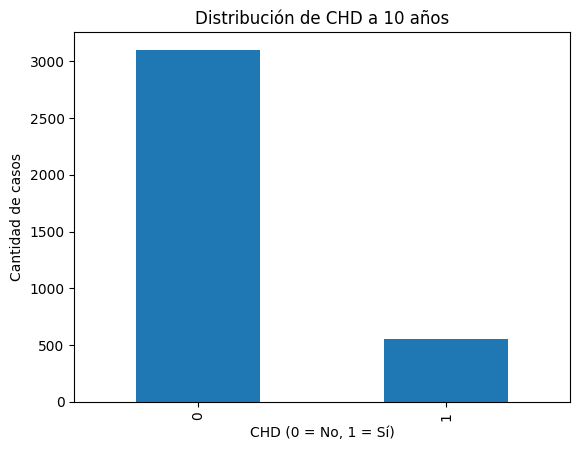
\includegraphics[width=0.65\linewidth]{CHDdist.png}
        \caption{Distribución de CHD a 10 años.}
        \label{CHD}
    \end{figure}
    
    Los datos muestran que la edad promedio de los participantes en el estudio es de aproximadamente 49.6 años, con una desviación estándar de 8.6 años, lo que indica una dispersión moderada en torno a la media. La edad mínima registrada es de 32 años y la máxima de 70 años, por lo que el conjunto de datos representa principalmente a una población adulta de mediana edad y adulta mayor.
    
    El rango intercuartílico se extiende de 42 a 56 años, lo que significa que el 50\% central de los individuos se encuentra dentro de ese intervalo. Este comportamiento sugiere una distribución relativamente concentrada alrededor de la media, sin presencia de valores atípicos extremos. Dado que la cardiopatía coronaria suele asociarse con la edad, esta variable probablemente tendrá un peso significativo en la predicción del modelo.
    
    
    \begin{figure}[H]
        \centering
        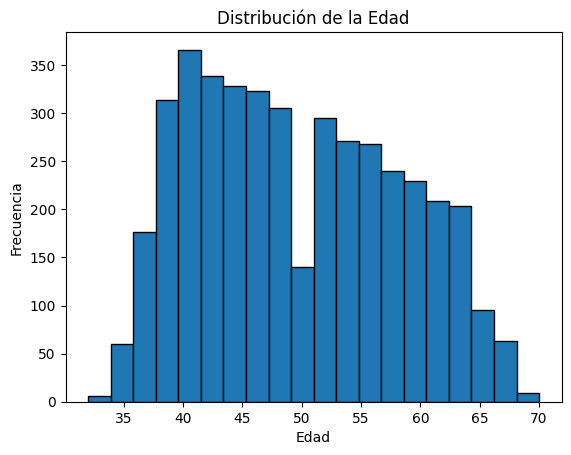
\includegraphics[width = 0.65 \linewidth]
        {age.png}
        \caption{Distribución de la Edad.}
        \label{age1}
    \end{figure}
    
    La distribución de la edad según la presencia de cardiopatía coronaria muestra una diferencia notable entre ambos grupos. Las personas que desarrollan la enfermedad en los siguientes diez años tienden a concentrarse en edades mayores, especialmente a partir de los 50 años, donde la curva correspondiente a los casos positivos presenta un incremento más marcado. En contraste, la población sin enfermedad muestra una distribución más uniforme y con menor densidad en los rangos altos de edad. Estos resultados sugieren que la edad es un factor de riesgo relevante para la cardiopatía coronaria, lo cual coincide con la evidencia clínica. La superposición de ambas distribuciones confirma que, aunque existe variabilidad entre individuos, el riesgo aumenta conforme avanza la edad, aportando información valiosa para el entrenamiento de los modelos predictivos.
    
    \begin{figure}[H]
        \centering
        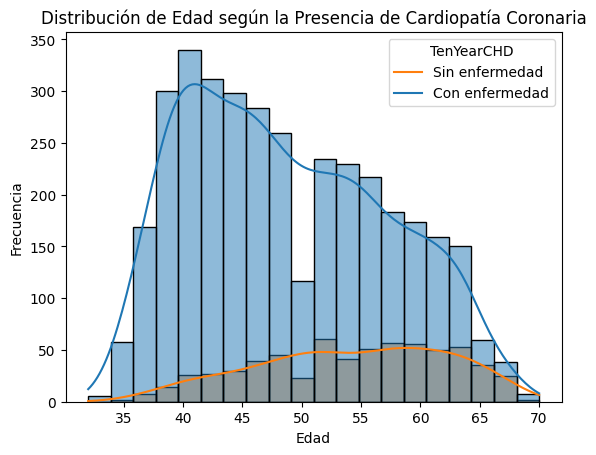
\includegraphics[width = 0.65 \linewidth]
        {age CHD.png}
        \caption{Distribución de edad según la presencia de Cardiopatía Coronaria.}
        \label{age2}
    \end{figure}
    
    \begin{figure}[H]
        \centering
        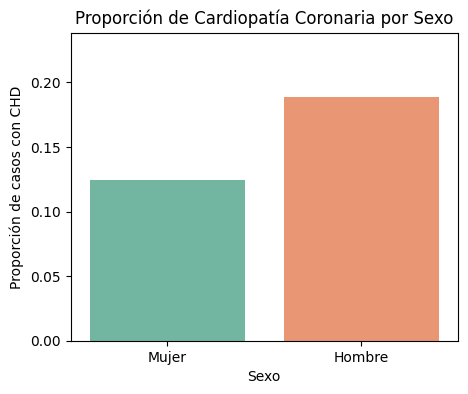
\includegraphics[width = 0.60 \linewidth]
        {Sex_CHD.png}
        \caption{Proporción de Cardiopatía Coronaria por Sexo.}
        \label{age3}
    \end{figure}


       Como parte de la exploración de los datos, se realizaron distintas gráficas para encontrar relaciones entre los datos que pudieran ser útiles para nuestra investigación, de las cuales se seleccionaron dos de las que consideramos más relevantes para incluirlas en este apartado.
    
        La primera gráfica a presentar, fue realizada usando los atributos \texttt{totChol} (nivel de colesterol), \texttt{sysBP} (presión sistólica) y \texttt{age} (edad), y se obtuvo la siguiente gráfica.
    
        \begin{figure}[H]
            \centering
            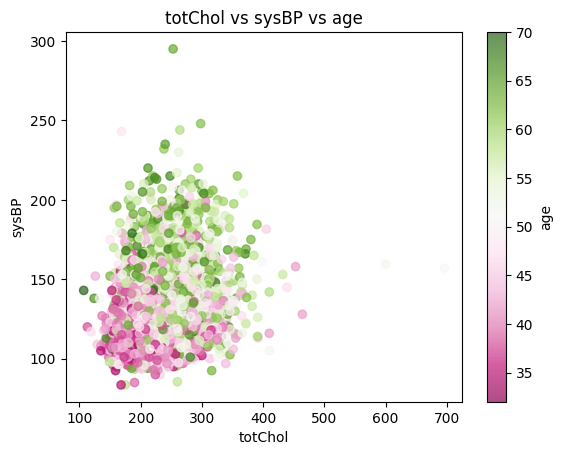
\includegraphics[width=0.7\linewidth]{totChol vs sysBP vs age.png}
            \label{fig:enter-label}
            \caption{Nivel de colesterol contra presión sistólica y edad.}
        \end{figure}
    
        Podemos encontrar que es frecuente que las personas mayores de 50 años presenten niveles elevados de colesterol, además de una presión sistólica elevada.
    
        La segunda gráfica fue realizada con los atributos \texttt{age} (edad), \texttt{totChol} (nivel de colesterol) y \texttt{TenYearCHD} (Riesgo de presentar la enfermedad en 10 años), y la imagen generada fue la siguiente:
        
       \begin{figure}[H]
           \centering
        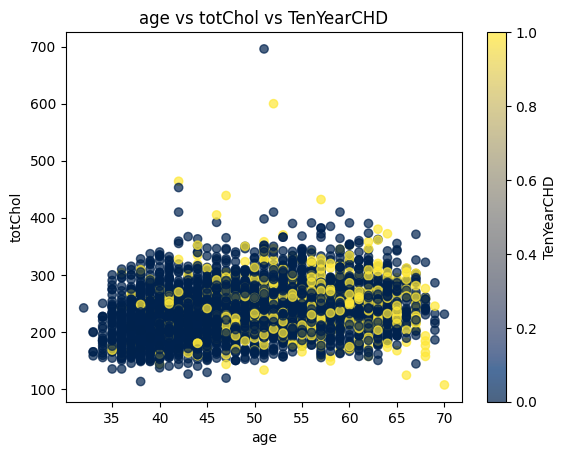
\includegraphics[width=0.7\linewidth]{age vs totChol vs TenYearCHD.png}
           \label{fig:enter-label}
           \caption{edad contra nivel de colesterol y Riesgo de presentar la enfermedad en 10 años.}
       \end{figure}
    
       Esta gráfica es la que consideramos como la más relevante, pues nos confirma algo que ha sido alertado por diversos profesionales de la salud: los factores de riesgo más importantes que podrían influir en que una persona enferme de CHD son la edad avanzada y los altos niveles de colesterol.
    
    Con el fin de identificar posibles relaciones entre las variables cuantitativas del conjunto de datos, se construyó una matriz de correlación. Esta herramienta permite observar qué tan fuertemente se asocian las variables entre sí, facilitando la detección de factores que podrían influir en la presencia de cardiopatía coronaria.
    
    \begin{figure}[H]
    \centering
        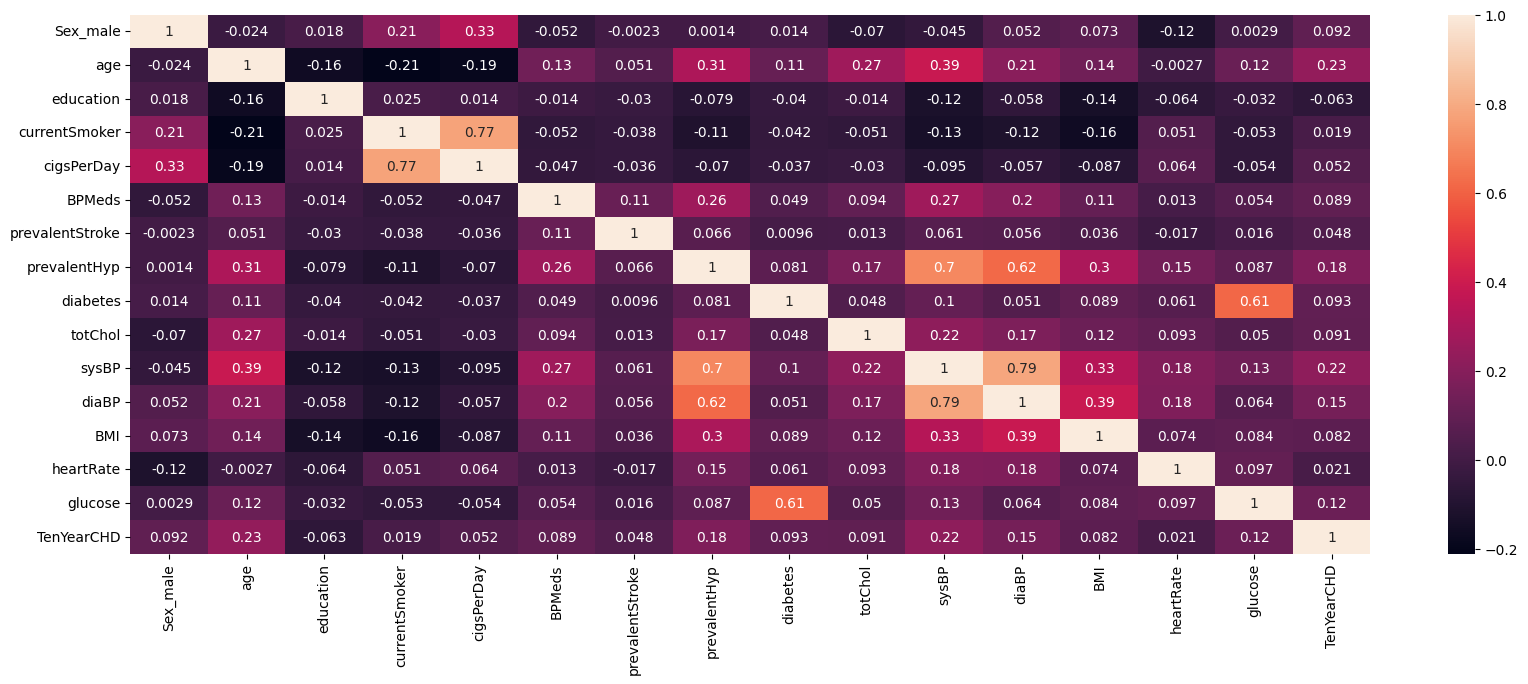
\includegraphics[width=1.0 \linewidth]{corrmatrix.png}
        \caption{Matriz de correlación.}
        \label{correl}
    \end{figure}

    \subsection{Regresión logística}

    Una vez realizado el análisis exploratorio y la identificación de las variables más relevantes, se procedió a la construcción del modelo de Regresión Logística, cuyo objetivo es predecir la probabilidad de desarrollar cardiopatía coronaria a 10 años. 

    Comenzamos importando las librerias necesarias, $\texttt{numpy}$ que sirve para crear vectores y matrices grandes multidimensionales, y funciones de alto nivel, $\texttt{scipy.optimize}$ para optimización, álgebra lineal, integración, interpolación, funciones especiales, FFT, procesamiento de señales y de imagen, resolución de ODEs, etc, $\texttt{statsmodel.api}$, una biblioteca de análisis y modelado de datos estadísticos, y $\texttt{sklearn}$ que incluye varios algoritmos de clasificación, regresión y análisis de grupos entre los cuales están máquinas de vectores de soporte, bosques aleatorios, Gradient boosting, K-means, entre otros.


    \begin{figure}[h!]
       \begin{center}
           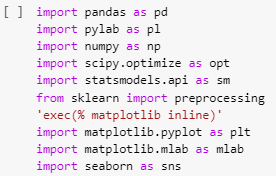
\includegraphics[width=0.4\linewidth]{librerias.png}
           \caption{Importación de librerías.}
            \label{fig:librerias}
        \end{center}
    \end{figure}

    Luego, se definieron como variables independientes aquellas que mostraron una relación significativa con la enfermedad, tales como la \textit{edad}, el \textit{sexo}, la \textit{frecuencia cardíaca}, el \textit{colesterol total}, la \textit{presión arterial sistólica} y la \textit{glucosa}. La variable dependiente corresponde a la presencia o ausencia de la enfermedad (\texttt{TenYearCHD}).
    
    Antes del entrenamiento, las variables independientes fueron normalizadas mediante la técnica StandardScaler, con el fin de garantizar que todas las características tuvieran una escala comparable. Posteriormente, los datos se dividieron en un conjunto de entrenamiento (70\%) y otro de prueba (30\%) para evaluar el desempeño del modelo, como se muestra en la siguiente imagen. 

    \begin{figure}[H]
    \centering
        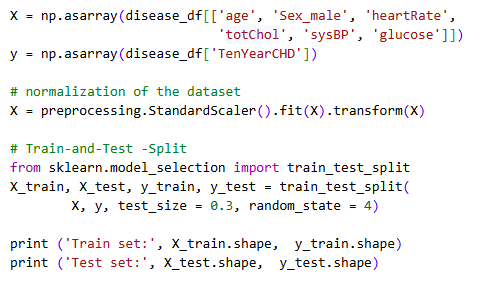
\includegraphics[width = 0.65 \linewidth]{variables.png}
        \caption{Definicion de variables.}
        
    \end{figure}


        \subsubsection{Resultados Del Modelo De Regresión Logística}
    
        Al usar los atributos \texttt{age}, \texttt{BPMeds}, \texttt{prevalentStroke}, \texttt{totChol}, \texttt{diabetes}, \texttt{heartRate}; se obtuvieron resultados poco deseables, presentando un nivel alto de error. La matriz de confusión asociada a dicha prueba es la siguiente: 
    
        \begin{figure}[H]
            \centering
            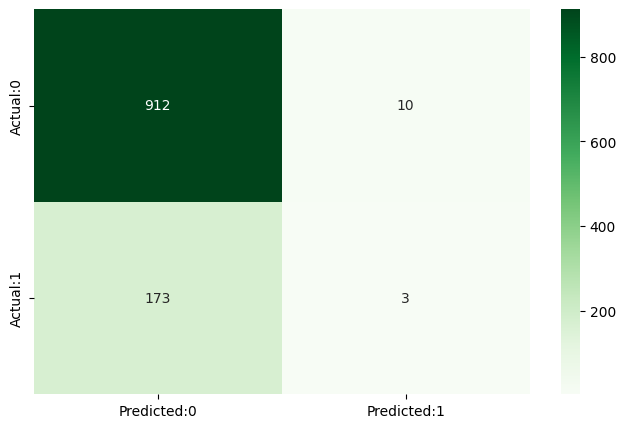
\includegraphics[width=0.75\linewidth]{Matriz2.png}
            \caption{Matriz de confusión de la regresón logística.}
            \label{fig:placeholder}
        \end{figure}
    
    
        \begin{figure}[H]
            \centering
            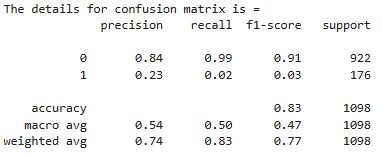
\includegraphics[width=0.55\linewidth]{Datos 2.png}
            \caption{Reporte de clasificación.}
            \label{fig:enter-label}
        \end{figure}
    
        Los resultados obtenidos a partir de la matriz de confusión y las métricas de evaluación muestran que el modelo de regresión logística presenta un buen desempeño general en términos de exactitud, alcanzando un valor de 0.83. Para la clase 0 (ausencia de enfermedad coronaria), el modelo obtiene valores altos de precisión (0.84), recall (0.99) y f1-score (0.91), lo que indica una alta capacidad para identificar correctamente a los pacientes que no presentan la enfermedad.
    
        Sin embargo, para la clase 1 (presencia de enfermedad coronaria), el desempeño del modelo es considerablemente menor, con una precisión de 0.23, un recall de 0.02 y un f1-score de 0.03. Esto sugiere que el modelo tiene dificultades para identificar correctamente los casos positivos, clasificando la mayoría de ellos como negativos. Este comportamiento puede atribuirse al desbalance entre las clases, ya que el número de observaciones correspondientes a la clase 0 es significativamente mayor que el de la clase 1.
        
        En conjunto, aunque el modelo presenta una exactitud elevada, las métricas por clase evidencian la necesidad de considerar estrategias adicionales para mejorar la detección de casos positivos, especialmente en un contexto médico donde los falsos negativos pueden tener consecuencias relevantes.
    
        Por el contrario, al utilizar los atributos age, Sexmale, heartRate, totChol, sysBP, glucose; se obtuvieron los resultados con mayor exactitud pero aún con deficiencias. La matriz de confusión obtenida es la siguiente:
    
         \begin{figure}[H]
         \centering
            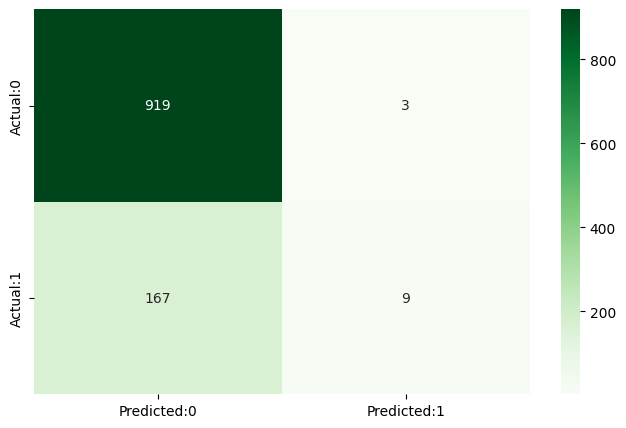
\includegraphics[width=0.75\linewidth]{Matriz1.png}
            \label{rl2mc}
            \caption{Matriz de Correlación de la segunda regresión logística.}
        \end{figure}
    
         \begin{figure}[H]
            \centering
            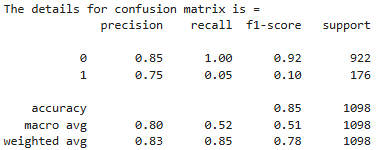
\includegraphics[width=0.55\linewidth]{Datos 1.png}
            \caption{Reporte de clasificación de la segunda regresión logística.}
            \label{rcrl2}
        \end{figure}
    
        La evaluación del modelo mediante la matriz de confusión y las métricas (figura \ref{rl2mc} y figura \ref{rcrl2}) de desempeño muestra una exactitud del 0.85, lo que indica un buen rendimiento global del clasificador. Para la clase 0 (ausencia de enfermedad coronaria), el modelo alcanza valores elevados de precisión (0.85), recall (1.00) y f1-score (0.92), evidenciando una excelente capacidad para identificar correctamente a los pacientes que no presentan la enfermedad.
        
        En el caso de la clase 1 (presencia de enfermedad coronaria), se observa una mejora en la precisión, alcanzando un valor de 0.75; sin embargo, el recall continúa siendo bajo (0.05), con un f1-score de 0.10. Esto indica que, aunque cuando el modelo predice la presencia de la enfermedad suele acertar, sigue detectando únicamente una pequeña proporción de los casos positivos reales. Este comportamiento sugiere que el modelo mantiene una fuerte tendencia a clasificar las observaciones como pertenecientes a la clase mayoritaria, lo cual puede atribuirse al desbalance en el conjunto de datos.
        
        En este contexto, a pesar de la mejora en algunas métricas, resulta necesario considerar ajustes adicionales para incrementar la sensibilidad del modelo hacia la clase positiva, especialmente debido a la relevancia clínica de detectar oportunamente los casos de enfermedad coronaria.
    
    \subsection{Árbol de decisión}
    
    Antes de entrenar el modelo de árbol de decisión, fue necesario preparar nuevamente los datos. En primer lugar, se definió la variable dependiente (\texttt{TenYearCHD}), que representa la presencia o ausencia de cardiopatía coronaria, y se eliminaron estas etiquetas del conjunto de variables independientes (\texttt{X}). Posteriormente, se codificaron las variables categóricas —como el sexo— mediante valores numéricos, de manera que pudieran ser interpretadas por el modelo. Finalmente, se aplicó un proceso de imputación para manejar los valores faltantes, sustituyendo los registros vacíos por el valor anterior disponible (forward fill), con el objetivo de mantener la coherencia y la completitud del conjunto de datos antes del entrenamiento.
    
    \begin{figure}[H]
        \centering
        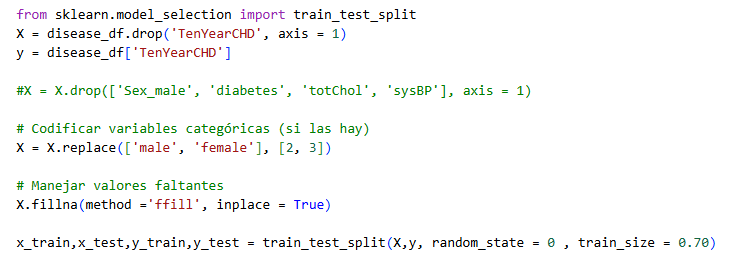
\includegraphics[width = 0.9 \linewidth]
        {DT_vari.PNG}
        \caption{Definición de variables para el árbol de decisión.}
        \label{DTvari}
    \end{figure}
        
    Como podemos ver en la imagen \ref{DTvari}, para el modelo de árbol de decisión, se definieron las variables independientes (\texttt{X}) y la variable dependiente (\texttt{y}). En este caso, X está conformada por todas las características del conjunto de datos, excepto la variable objetivo, mientras que y corresponde a la variable \texttt{TenYearCHD}, que indica la presencia o ausencia de cardiopatía coronaria. Esta separación permite que el modelo aprenda patrones a partir de las variables predictoras y posteriormente pueda estimar la probabilidad de que un individuo desarrolle la enfermedad. De este modo, el árbol de decisión utilizará todos los atributos disponibles para construir reglas jerárquicas que dividan los datos en función de los valores que mejor separen las clases. De igual manera,  los datos se dividieron en un conjunto de entrenamiento (70\%) y otro de prueba (30\%) para evaluar el desempeño del modelo.
        
    \begin{figure}[H]
        \centering
        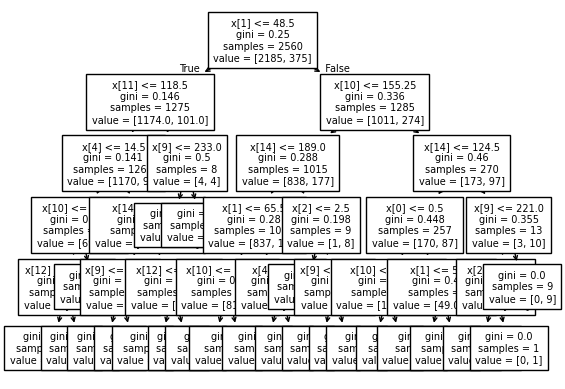
\includegraphics[width=0.8\linewidth]{Arbol_Visual.png}
        \caption{Entrenamiento del modelo de árbol de decisión.}
        \label{visualizacion}
    \end{figure}


        \subsubsection{Resultados del Árbol de Decisión}

         El modelo de árbol de decisión permitió clasificar los datos de manera clara, mostrando qué variables influyeron más en la predicción. A través de las divisiones sucesivas del árbol, se observó cómo el modelo fue estableciendo reglas basadas en los valores de las características más relevantes. Esto facilitó interpretar los patrones dentro del conjunto de datos y visualizar la relación entre las variables y la categoría final predicha. En general, el árbol ofreció una representación visual sencilla y explicativa del proceso de clasificación, destacando la importancia de las variables que mejor separaron a los distintos grupos.
         A continuación se presentan la matriz de confusión y la matriz de métricas obtenidas a partir del modelo de árbol de decisión. Estos resultados permiten evaluar el desempeño del modelo al comparar las predicciones realizadas con los valores reales, mostrando el número de aciertos y errores en cada categoría, así como las principales métricas de clasificación como la precisión, la exhaustividad y la puntuación F1.
        
        \begin{figure}[H]
            \centering
            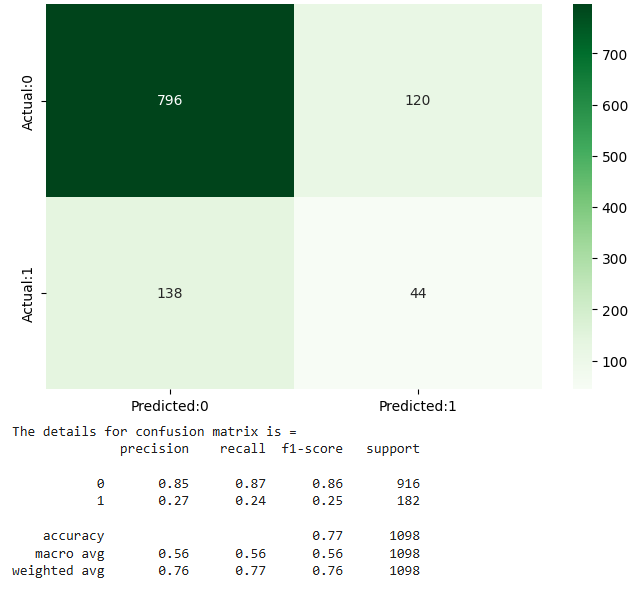
\includegraphics[width = 0.8 \linewidth]
            {Arbol_MC.PNG}
            \caption{Mátriz de confusión y métricas del modelo de árbol de decisión.}
            \label{DescDatos}
        \end{figure}
        
        El modelo de árbol de decisión alcanzó una exactitud (accuracy) del 77\%, lo que representa una ligera disminución respecto a la regresión logística, aunque con un mejor equilibrio en la detección de ambas clases. Para la clase 0 (sin enfermedad), el modelo mantiene un desempeño sólido, con precision y recall de 0.85 y 0.87, respectivamente. En contraste, para la clase 1 (con riesgo de cardiopatía coronaria), las métricas mejoran levemente en comparación con la regresión logística: la precision es de 0.27 y el recall de 0.24, lo que indica que el árbol logra identificar un número mayor de casos positivos, aunque todavía de forma limitada.
        La matriz de confusión muestra que el modelo clasifica correctamente 796 casos sin enfermedad y 44 con enfermedad, pero aún confunde una cantidad considerable de positivos y negativos.
        
        En general, el árbol de decisión captura mejor la complejidad no lineal de los datos, aunque su rendimiento sigue condicionado por el desequilibrio en el número de muestras por clase, aspecto que podría optimizarse mediante técnicas de resampling o ajustes de hiperparámetros. 

\newpage
\section{Conclusiones}

En el presente trabajo se aplicaron técnicas de aprendizaje supervisado para la detección del riesgo de enfermedad coronaria a diez años, utilizando los modelos de regresión logística y árbol de decisión. A partir del análisis exploratorio de datos y de la implementación de ambos algoritmos, fue posible evaluar su desempeño y comparar sus capacidades para abordar un problema de clasificación binaria en un contexto médico.

Los resultados obtenidos con la regresión logística mostraron una buena exactitud global; sin embargo, el modelo presentó dificultades para identificar correctamente los casos positivos, lo que se reflejó en valores bajos de recall para la clase correspondiente a la presencia de enfermedad coronaria. Este comportamiento evidenció el impacto del desbalance entre clases y puso de manifiesto que la exactitud, por sí sola, no es una métrica suficiente para evaluar modelos aplicados al ámbito de la salud.

Por su parte, el árbol de decisión permitió capturar relaciones no lineales entre las variables y mejoró la capacidad de detección de la clase positiva en comparación con la regresión logística, aunque su desempeño general fue inferior en términos de exactitud. A pesar de esta mejora, el número de falsos negativos continuó siendo significativo, lo cual representa una limitación importante desde el punto de vista clínico.

En conjunto, ambos modelos mostraron ventajas y limitaciones específicas, destacando la importancia de seleccionar métricas de evaluación adecuadas y de considerar el contexto del problema. En aplicaciones médicas como la detección de enfermedades cardiovasculares, resulta fundamental priorizar la capacidad del modelo para identificar correctamente los casos positivos. Como trabajo futuro, se propone explorar estrategias para el manejo del desbalance de clases y la optimización de los modelos, con el objetivo de mejorar su desempeño y su utilidad en escenarios reales.

Como trabajo futuro, se sugiere explorar estrategias que permitan mejorar la detección de los casos positivos de enfermedad coronaria, dado el desbalance presente en el conjunto de datos. Entre estas estrategias se encuentra el ajuste del umbral de decisión en los modelos de clasificación, así como el uso de técnicas de balanceo de clases, tales como sobremuestreo, submuestreo o métodos basados en generación sintética de datos.

Asimismo, sería conveniente evaluar el desempeño de otros algoritmos de aprendizaje supervisado, como bosques aleatorios o máquinas de soporte vectorial, los cuales podrían capturar relaciones más complejas entre las variables. De igual forma, la implementación de validación cruzada permitiría obtener estimaciones más robustas del desempeño de los modelos.

Finalmente, se propone incorporar métricas de evaluación adicionales, como la curva ROC, el área bajo la curva (AUC) y la sensibilidad, las cuales resultan especialmente relevantes en el contexto médico, donde la detección temprana de la enfermedad es prioritaria.


\newpage

\section{Referencias}

\begin{enumerate}
    \item What Is Machine Learning? Definition, Types, Applications, and Trends. \\
    \url{https://www.spiceworks.com/soft-tech/what-is-ml/}.
    \item What Is General Artificial Intelligence (AI)? Definition, Challenges, and Trends. \\
    \url{https://www.spiceworks.com/tech/iot/articles/what-is-ailing-iot-at-scale/}.
    \item What Is Linear Regression?  \\
    \url{https://www.spiceworks.com/soft-tech/what-is-linear-regression/}
    \item Linear Regression vs. Logistic Regression \\
    \url{https://www.spiceworks.com/soft-tech/linear-regression-vs-logistic-regression/}
    \item What Is Logistic Regression? Equation, Assumptions, Types, and Best Practices \\
    \url{https://www.spiceworks.com/soft-tech/what-is-logistic-regression/}
    
    
\end{enumerate}

\newpage

El presente documento ha sido elaborado exclusivamente como parte del reporte de Servicio Social de Estudios Técnicos Especializados por parte de la Escuela Nacional Preparatoria de la UNAM. Queda estrictamente prohibida su reproducción, distribución o utilización para fines distintos a los académicos que le dieron origen.

Bajo la dirección y supervisión de:


\begin{center}
\vspace{5cm}
%\rule{7cm}{0.4pt}\\%
   Ingrid Midory Monterroso Alfaro \\
Responsable del Programa de Servicio Social y Práctica Profesional\\  
\textit{Data Minds. Laboratorio de Inteligencia Artificial y Machine Learning} 
\end{center}

\end{document}